\documentclass[11pt,a4paper]{article}
\usepackage[margin=21mm,top=22mm,bottom=22mm,headheight=13pt,headsep=8mm,footskip=11mm]{geometry}
\usepackage{fontspec}
\setmainfont{EBGaramond12-Regular.ttf}[Path=/usr/share/fonts/truetype/ebgaramond/,BoldFont=EBGaramond12-Bold.ttf,ItalicFont=EBGaramond12-Italic.ttf,BoldItalicFont=EBGaramond12-Bold.ttf,Numbers=OldStyle]
\setsansfont{Inter}
\setmonofont[Scale=.85]{DejaVu Sans Mono}
\usepackage{amsmath,amssymb,booktabs,tabularx,array,graphicx,xcolor,hyperref,fancyhdr,titlesec,enumitem,multicol}
\definecolor{cardinal}{HTML}{8C1515}
\definecolor{charcoal}{HTML}{262526}
\definecolor{muted}{HTML}{666665}
\definecolor{sand}{HTML}{B18A5A}
\definecolor{ice}{HTML}{F0F0ED}
\hypersetup{colorlinks=true,linkcolor=cardinal,urlcolor=cardinal,bookmarksnumbered=true,pdftitle={Xcelerate FC | Possession Inference Technical Report},pdfauthor={Xcelerate FC}}
\setlength{\parindent}{0pt}
\setlength{\parskip}{5pt}\linespread{1.075}
\renewcommand{\arraystretch}{1.13}
\setlist[itemize]{leftmargin=16pt,topsep=2pt,itemsep=2pt,parsep=0pt}
\pagestyle{fancy}
\fancyhf{}
\fancyhead[L]{\sffamily\fontsize{7}{8}\selectfont\color{muted} XCELERATE FC}
\fancyhead[R]{\sffamily\fontsize{7}{8}\selectfont\color{muted} MORE THAN A HACK 2027}
\renewcommand{\headrulewidth}{0pt}
\fancyfoot[L]{\sffamily\fontsize{7}{9}\selectfont\color{muted} Possession inference | Technical report | 15 November 2026}
\fancyfoot[R]{\sffamily\fontsize{8}{9}\selectfont\color{cardinal}\thepage\, / \,7}
\renewcommand{\footrulewidth}{0pt}
\newcommand{\sectionlead}[2]{\vspace{3pt}{\sffamily\fontsize{9}{11}\selectfont\color{cardinal}\bfseries #1}\par\vspace{4pt}{\sffamily\fontsize{20}{23}\selectfont\bfseries\color{charcoal} #2}\par\vspace{4pt}{\color{cardinal}\rule{17mm}{1.1pt}}\vspace{8pt}\par}
\newcommand{\smallhead}[1]{\vspace{6pt}{\sffamily\fontsize{10}{12}\selectfont\bfseries\color{charcoal} #1}\par\vspace{1pt}}
\newcommand{\micro}[1]{{\sffamily\fontsize{7.5}{10}\selectfont\color{muted}#1}}
\newcommand{\caplabel}[1]{{\sffamily\fontsize{7.2}{9}\selectfont\color{muted}#1}}
\newcommand{\metric}[2]{\begin{minipage}[t]{.29\linewidth}\sffamily\fontsize{20}{23}\selectfont\bfseries\color{cardinal} #1\par\vspace{3pt}\fontsize{8}{10}\selectfont\color{muted} #2\end{minipage}}
\renewcommand{\emph}[1]{{\itshape #1}}
\begin{document}
% PAGE 1: COVER
\thispagestyle{empty}
\vspace*{18mm}
{\sffamily\fontsize{10}{12}\selectfont\bfseries\color{cardinal} XCELERATE FC\hspace{5mm}|\hspace{5mm} MORE THAN A HACK 2027}\par
\vspace{28mm}
{\sffamily\fontsize{33}{36}\selectfont\bfseries\color{charcoal} Who Has the Ball?}\par
\vspace{5mm}
{\sffamily\fontsize{20}{25}\selectfont\color{charcoal} A sequence-aware system for football possession inference}\par
\vspace{9mm}
{\color{cardinal}\rule{38mm}{1.7pt}}\par
\vspace{15mm}
\begin{minipage}{.88\linewidth}
\fontsize{12}{16}\selectfont
We developed a reproducible pipeline that converts automatic tracking and tactical events into frame-level home, away and dead-ball labels. Our experiments moved from nearest-player geometry to temporal decoding, then to explicit ball-control memory and multi-scale fusion. We selected the final model using five external matches, checked it once on a separate external match and kept the competition's public five-minute labels out of model selection.
\end{minipage}
\vspace{20mm}
{\sffamily\fontsize{9}{11}\selectfont\color{muted} VERIFIED RESULTS}\par\vspace{5mm}
\metric{0.4823}{External proxy spellF1\\5 development matches}\hfill
\metric{0.4078}{External proxy spellF1\\fresh holdout}\hfill
\metric{356}{Predicted H/A possessions\\complete competition video}\par
\vfill
{\sffamily\fontsize{9}{11}\selectfont\bfseries TEAM MEMBERS}\par\vspace{3mm}
{\fontsize{11}{15}\selectfont
KAMBIRE Eric\quad LARAISSE Hamza\quad BELEMCOABGA Falleiz Rostem\par
BATIONO Max Dieudonn\'e Nathan\quad SIMBORO Rydouane\par}
\vspace{10mm}
\micro{Public code: \href{https://github.com/khalifasimboro/Xcelerate-FC}{github.com/khalifasimboro/Xcelerate-FC} \hfill Submission date: November 2026}\par
\clearpage
% PAGE 2
\sectionlead{01 / QUESTION AND DATA}{From video frames to possessions}
\smallhead{Why this is a sequence problem}
The task covers a 199,319-frame tactical video at 25 frames per second, with labels \textbf{H} (Barcelona), \textbf{A} (Athletic Club), \textbf{D} (ball not in play) and \textbf{X} (ungraded interval). A possession is a continuous H or A spell, not a vote taken independently at every frame. The competition ranks predictions with \emph{spellF1}: predicted and reference possessions are matched one to one by temporal intersection over union at thresholds 0.3, 0.4, 0.5, 0.6 and 0.7. We therefore optimized temporal consistency rather than isolated frame accuracy.

\smallhead{M1. Establishing a data pipeline and the first observation rule}
We aligned automatic tracking to video frames, resolved home and away players from the team-association data, and read automatic tactical tags. Homography-based field coordinates let us compute the nearest player and team to the ball. The first rule used that distance, with simple priors for tactical events and the dead-ball state. This was a necessary baseline, but it could change possession during passes or contested balls because the nearest player is not always the ball's controller.

Our first temporal model turned these features into three unnormalized observation scores, then decoded the most plausible H/A/D path with Viterbi. These scores were designed heuristically; we did not claim to have trained a probabilistic hidden Markov model on competition labels.

\smallhead{Assets and their boundaries}
\begin{tabularx}{\linewidth}{@{}>{\bfseries}p{30mm}X@{}}
\toprule
Asset & How we used it\\
\midrule
Competition tracking & Ball and player coordinates, distance, visibility and approximate speed\\
Automatic tactical tags & Offensive context and candidate restart types, subject to timestamp uncertainty\\
Team association & Consistent home/away identification\\
Competition video & Inspection and alignment checks, not manual possession annotation\\
SkillCorner open data & External H/A-labelled possession tests on different football matches\\
\bottomrule
\end{tabularx}
\vspace{3mm}
\smallhead{What was never used as training data}
The supplied Barcelona--Athletic game had no human labels added by our team. The published five-minute reference was reserved for pipeline checks only. We did not use human-produced event labels from another provider about this competition game. We used automatic features from the game, including deterministic memory and unsupervised preprocessing, in accordance with the competition rules.
\vfill
\caplabel{Sources: More Than a Hack 2027, RULES.md, EVALUATION.md and SUBMISSION.md.}\par
\clearpage
% PAGE 3
\sectionlead{02 / TEMPORAL MODELING}{Making predictions persist}
\smallhead{M2. Why Viterbi became the first improvement}
The basic model produced too many short possession spells when the ball crossed between players. We introduced transition costs so that a change from H to A needed stronger evidence than staying in the current state. We also treated H/A exchanges and transitions to or from D differently.

The initial decoding costs were \((13,10,7)\). We then tested \((23,17,11)\), called \texttt{switch\_strong}. The higher penalties made possessions less fragmented without requiring labels from the competition game. We also tried temperature scaling of observation scores; raising temperature to three made the decoder more persistent, but could preserve the wrong team for too long.

\smallhead{An external comparison before adding new football rules}
The first five SkillCorner development matches, with IDs 1886347, 1899585, 1925299, 1996435 and 2006229, were evaluated in a match-wise protocol. Their labels identify H/A possession only where \texttt{possession.group} is known. We adapted 10 Hz tracking to the time-scale of our 25 Hz decoder, without treating unknown possession labels as D.

\begin{center}
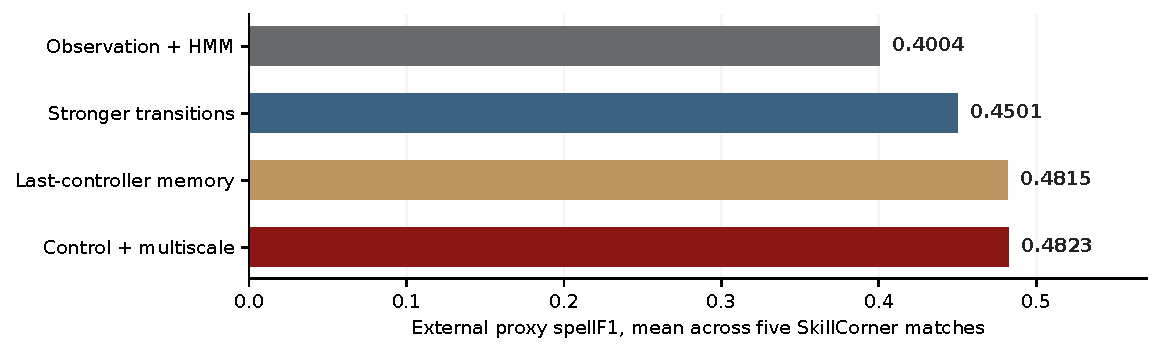
\includegraphics[width=.91\linewidth]{figures/XC_report_progression.pdf}\par
\caplabel{Figure 1. Progressive mean proxy spellF1 on five external matches. These are external proxy metrics, not private competition scores.}
\end{center}
\smallhead{Decision after M2}
\texttt{switch\_strong} achieved \textbf{0.4501} mean external proxy spellF1, compared with \textbf{0.4004} for the initial HMM-style baseline. Increasing temporal persistence was helpful, but not sufficient. The model still lacked an explicit representation of who last controlled the ball when it became temporarily free or invisible.

\vfill
\caplabel{Interpretation: each point above is a match-level summary, not a count of independent video frames.}\par
\clearpage
% PAGE 4
\sectionlead{03 / FOOTBALL STRUCTURE}{From proximity to actual control}
\smallhead{M3. Remember the last credible controller}
A pass does not automatically transfer possession to the team whose player becomes momentarily closest to the moving ball. We added a controller candidate only when the ball was observed, a player was within 1.8 m, the opposing team did not have a player in that same radius, and the observation persisted for at least five frames at 25 Hz. Fast balls above 16 m/s were not allowed to initiate a new control. The last credible controller could then support its team's score for up to ten seconds, with exponentially decreasing weight:
\[
\Delta z_{\mathrm{team}}(t)=1.5\,\exp(-a(t)/6),\qquad 0\leq a(t)\leq10\ \mathrm{s}.
\]
This is a confidence heuristic, not evidence that the same player physically touched the ball for ten seconds. We reset that memory at recognized restart boundaries. Short, two-sided tracking gaps were interpolated for geometry, but an interpolated ball location never created a new observed control.

\smallhead{Ablation before fusion}
We next introduced simultaneous proximity by opposing players as a duel indicator and large ball-acceleration changes as possible touches. Both were treated as weak evidence. We then blended controller-aware and multi-scale observations before using the strong transition decoder. This preserved the last-controller mechanism while adding smoother geometry over several time windows.

\begin{tabularx}{\linewidth}{@{}>{\raggedright\arraybackslash}Xrr@{}}
\toprule
External model, five-match development set & Proxy spellF1 & H/A macroF1\\
\midrule
\texttt{switch\_strong} & 0.4501 & 0.7977\\
\texttt{control\_strong} & 0.4815 & 0.8195\\
\texttt{control\_duel\_strong} & 0.4808 & 0.8194\\
\texttt{control\_touch\_strong} & 0.4809 & 0.8194\\
\textbf{\texttt{fusion\_control\_multiscale}} & \textbf{0.4823} & \textbf{0.8200}\\
\bottomrule
\end{tabularx}
\vspace{3mm}
The controller feature produced the main gain. Duel and touch cues did not produce a reliable further improvement in this evaluation, so we kept them as traceable alternatives rather than claiming they were essential. The multiscale fusion delivered the highest robust cross-match score, although the gain over controller-only was small.

\smallhead{What the fusion actually combines}
The selected model blends the controller-enhanced H/A observations with a Gaussian-smoothed, multi-scale context signal. Viterbi then decodes a consistent sequence using the stronger transition penalties. A micro-spell postprocessor was tested separately, but its external scores matched the unprocessed fusion. The extra postprocessing was therefore not needed for the submitted model.
\clearpage
% PAGE 5
\sectionlead{04 / INTERRUPTIONS AND LEARNED FEATURES}{What we tested, and what we did not claim}
\smallhead{M4. A physically motivated dead-ball branch}
Our initial D score used tactical set-piece tags, nearest-player distance, low team speed, ball visibility and whether the ball appeared outside normalized field bounds. This could confuse missing observations with a stoppage. We developed a second score, \texttt{D\_V2}, using confirmed boundary crossings, restart preparation, ball immobility near a line, temporary stop memory, active-play evidence and restart motion. In V2, an invisible ball alone gives no positive evidence for D.

On the competition input, \texttt{D\_V2\_strong} predicted more stoppages and reduced the share of its D predictions made while the ball was invisible. However, in external SkillCorner tests its H/A proxy spellF1 was \textbf{0.4424} and its false-D rate on known H/A frames was \textbf{0.6209\%}, compared with \textbf{0.0317\%} for \texttt{switch\_strong}. The external dataset does not provide a trustworthy complete set of D labels. We could measure spurious D calls on known live possessions, but not dead-ball recall. We therefore kept V2 experimental rather than allowing a public five-minute diagnostic to determine the final D policy.

\smallhead{A separate test of a tabular foundation model}
We also screened \texttt{TabICLv2}, using external H/A examples from other matches. Its scikit-learn-style interface takes numerical tracking features and predicts class probabilities. On five held-out external match samples, TabICLv2 exceeded a classical HistGradientBoosting baseline in each sample. For example, their H/A macroF1 values were 0.7560 versus 0.7447 on match 1886347 and 0.7709 versus 0.7550 on match 1925299.

These were balanced-sample classification tests, not full-sequence spellF1 tests. The full five-match temporal evaluation of TabICL fusion was not run. We did \textbf{not} include TabICL in the final eligibility list. Its probabilities are a possible future addition to H/A evidence, not proof of better end-to-end possession spells.

\smallhead{Restart semantics and unimplemented claims}
We recognized restart types such as throw-ins, corners, goal kicks, free kicks and kickoffs, and cleared controller memory at their boundaries. We did not assume an ambiguous \texttt{Team} attribute always identified the awarded team. We did not claim referee-whistle detection, calibrated homography reprojection uncertainty or full video-based ball-contact recognition, because the required measurements were not available with sufficient reliability.
\vfill
\caplabel{No labelled data from the competition match was used to learn or tune either the D branch or the foundation-model screening.}\par
\clearpage
% PAGE 6
\sectionlead{05 / EXTERNAL VALIDATION AND LOCK}{The evidence behind our final choice}
\smallhead{Five development matches, one locked model}
We used a match-wise leave-one-match-out check. Each of the five selections chose \texttt{fusion\_control\_multiscale} using the other four matches, which limits dependence on one favorable game. Across all five, the model reached mean proxy spellF1 \textbf{0.4823} with standard deviation \textbf{0.0178}, and H/A macroF1 \textbf{0.8200}. Its decoder did not predict D on known H/A evaluation frames in this development set.

\begin{center}
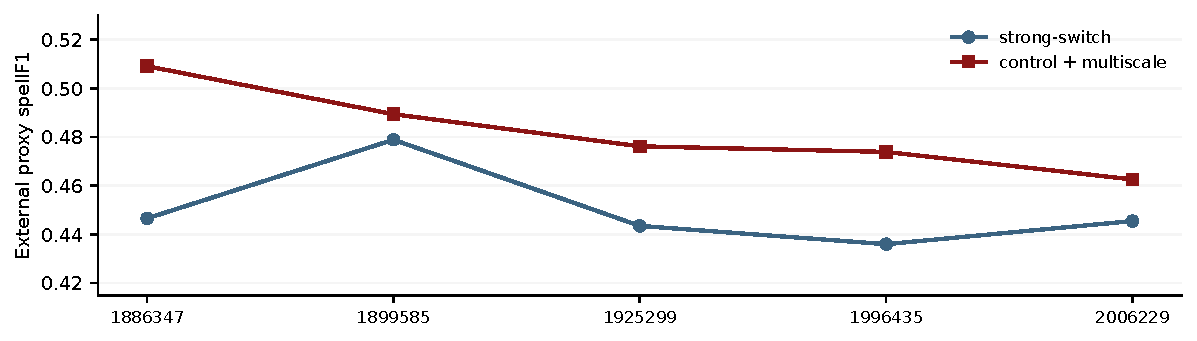
\includegraphics[width=.91\linewidth]{figures/XC_report_folds.pdf}\par
\caplabel{Figure 2. Model-wise results on each external development match. The model was chosen using external H/A evidence only.}
\end{center}
\smallhead{Independent external check after the model was locked}
We evaluated the selected configuration once on SkillCorner match \textbf{2017461}, which was excluded from development. It obtained proxy spellF1 \textbf{0.4078} and H/A macroF1 \textbf{0.7426}. Both are lower than the development averages, an important generalization warning. The known H/A subset covered 40.43\% of its frames. We did not revise the model in response to this result.

\smallhead{Public five-minute window, used only for alignment checks}
The competition provides 7,500 graded public frames containing 17 reference possessions. After locking our model externally, the official scorer produced \textbf{0.4108 spellF1}, \textbf{0.5076 macroF1} and 20 predicted possessions in this short window. The predicted F1 values were 0.7712 for H, 0.7518 for A and 0 for D. These checks exposed the limited dead-ball sensitivity of our chosen system; they did not trigger any coefficient change or model replacement. The five-minute sample is too short to act as a model-selection leaderboard and is explicitly prohibited for tuning by the rules.
\clearpage
% PAGE 7
\sectionlead{06 / DELIVERY}{Reproduction, limitations and compliance}
\smallhead{Final file and deterministic checks}
The selected implementation is \textbf{\texttt{fusion\_control\_multiscale}}, exported as \texttt{Xcelerate FC.csv}. It contains exactly \textbf{199,319} rows with columns \texttt{frame,label} and frame indices 0 through 199318. There are 92,388 H, 61,942 A, 4,527 D and 40,462 X entries. The prediction describes 356 H/A spells across the entire video. The required ungraded sections are X, and the pre-kickoff stretch of the second half is D. The CSV is 1,682,773 bytes and has SHA-256:
\begin{center}
{\ttfamily\fontsize{7.4}{9}\selectfont 6ae8a607a3c27bb96ec8da12b7e64326fb44765e8801ceb04f6844c21aa92c58}
\end{center}
The notebook's strict checks passed. The official \texttt{evaluation/validate\_submission.py} should also be executed against \emph{this exact file} before uploading it. A valid file format does not by itself validate possession accuracy.

\smallhead{How to reproduce our result}
\begin{enumerate}[leftmargin=17pt,topsep=2pt,itemsep=2pt]
\item Obtain the competition's data through authorized access. We mounted the assets as a \textbf{private Kaggle dataset} at \href{https://www.kaggle.com/datasets/erickambire/bar-data}{kaggle.com/datasets/erickambire/bar-data}. Access requires the owner to grant private-dataset collaborator permissions; the competition files are not public or redistributed.
\item Open the final Xcelerate notebook in Kaggle, attach the authorized competition dataset, enable Internet access only if downloading public SkillCorner/TabICL assets is required, and install the dependency requirements documented by the repository.
\item Run all cells in sequence with seed 2027. The development IDs are 1886347, 1899585, 1925299, 1996435 and 2006229; the reserved match is 2017461. TabICL screening is optional for reproduction of the selected non-TabICL model.
\item Verify that \texttt{MODEL\_TO\_EXPORT='AUTO'} resolves to \texttt{fusion\_control\_multiscale}. Regenerate the CSV, check its SHA-256, then run the official validator.
\end{enumerate}

\smallhead{Limitations and next experiments}
The main unresolved problem is D. Our selected model is supported by external H/A labels, not a dataset with complete stop-and-restart annotations. Ball visibility is imperfect, some restart timing is uncertain, and long occlusions make possession assignment ambiguous. The fresh holdout drop also shows that tracking and match context change across games. A next iteration needs independent labelled dead-ball sequences, richer referee and restart evidence, and a full temporal validation of TabICL before any new fusion is eligible for deployment.

\smallhead{Repository and technical sources}
\micro{\href{https://github.com/khalifasimboro/Xcelerate-FC}{Xcelerate FC public repository}. Reproduction code and documentation must be synchronized with this exact CSV before submission.}\par
\micro{\href{https://github.com/metrica-sports/more-than-a-hack-2027/blob/main/RULES.md}{Competition rules}, \href{https://github.com/metrica-sports/more-than-a-hack-2027/blob/main/EVALUATION.md}{evaluation protocol}, \href{https://github.com/metrica-sports/more-than-a-hack-2027/blob/main/SUBMISSION.md}{submission contract}.}\par
\micro{\href{https://github.com/SkillCorner/opendata}{SkillCorner open data}, external tracking and possession-group labels. TabICLv2 open pretrained model, used for screening only.}\par
\vfill
{\sffamily\fontsize{8}{11}\selectfont\color{cardinal}\bfseries XCELERATE FC \hfill 17 NOVEMBER 2026, 23:59 CET SUBMISSION DEADLINE}\par
\end{document}
